
\documentclass{beamer}

% Options are:
% Language Used:
% en - British English
% de - Standard German
% cy - Welsh
\usetheme{Redrose}


\module{NRG.AI4ME} % need to add this
\role{PhD Candidate}
\email{t.swarbrick}
% Need to reference a Collegue?
\acknowledge{ Dr Haris Rotsos, Prof Nick Race}
\title{Self-optimising distributed encoding nodes}
\author{Thomas Swarbrick}

\begin{document}
\maketitle
\section{Object Based Media}
\subsection{Traditional}
\begin{frame}[t]{Object Based Media}{A Static Approach to Objects}
  \begin{alertblock}{What is an object in object based media?}
    \begin{itemize}
\item Customisation of Characteristic, but the meta characteristics remain constant.
      \item Large customisable overlap, but not computationally feasible on the client-side.
    \end{itemize}

  \end{alertblock}
  \pause
  \begin{exampleblock}{Traditional Approach}
    \begin{itemize}
\item Changeable T-shirt colour
\item Geographically Specific Weather Map
    \end{itemize}

  \end{exampleblock}
  \pause
  But..
  \pause
    \begin{itemize}
\item Fixed in scope
      \item Susceptible to compute cost constraints.
    \end{itemize}
    \pause

\end{frame}
  \subsection{Dynamic Objects}
  \begin{frame}[t]{Object Based Media}{Encoder streams as Objects}
    Bring the Object Based Media (OBM) principle lower down the tool-chain.

    Most Compression Algorithms, make use of the 2D DCT II/III as part of their compression/analysis (Think MPEG).

    \begin{theorem}
      \emph{let} position be time-series \emph{like} such that.
      \[A = \{S^{A}_{0}\cdots S^{A}_{n}\}, B = \{S^{B}_{0}\cdots S^{B}_{m}\}\]
      where for a given object $S_{x}$ assume. \[ S_{x} \in A, S_{x} \in B\]
      \[  A =\{S_{x} | \Sigma_{1} \}, B = \{S_{x} | \Sigma_{2}\}\]
      such that.
      \[\Sigma_{1} \not\subset B, \Sigma_{2} \not\subset A\]
      \pause
     But how do you identify $S_{X}$? No idea.
    \end{theorem}
  \end{frame}

  \begin{frame}[t]{Object Based Media}{Encoder streams as Objects}
    \begin{theorem}
      Assume $S_{x}$ is identified, and we remove signal $S_{x}$ from the sets.
      \[ A \not= \sigma(B) + \Sigma_{1}, B \not= \sigma(A) + \Sigma_{2}\]

      i.e. A and B e are no longer correlated signals.

      So take some other set C. \[ C = \{S^{C}_{0}\cdots S^{C}_{p}\}\]

      assume $S_{y}$ is such that,

      \[  S_{y} \in B,  S_{y} \in C, S_{y} \not\in A, S_{y} \not\in S_{x}\]

      \[ B = \Sigma_{2}= \{S_{y}|\Sigma_{3}\}, C = \{S_{y}|\Sigma_{4}\}\]

      Figuring out if $S_{y}$ is not in A or $S_{x}$? No Idea.
    \end{theorem}
  \end{frame}

  \begin{frame}[t]{Object Based Media}{Encoder streams as Objects}
    \vspace{.5cm}
      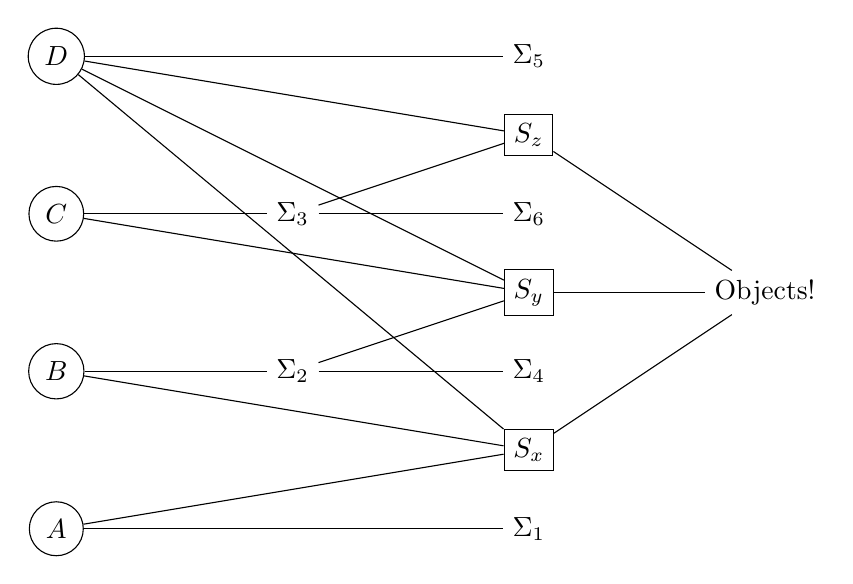
\begin{tikzpicture}
        \node at (0,0) [circle,draw] (A) {$A$};
        \node at (6,1) [rectangle,draw] (sx) {$S_{x}$};

        \node at (0,2) [circle,draw] (B) {$B$};
        \draw (A) -- (sx);
        \draw (B) -- (sx);

        \pause
        \node at (6,3) [rectangle,draw] (sy) {$S_{y}$};
        \node at (6,0) [] (sig1) {$\Sigma_{1}$};
        \node at (3,2) [] (sig2) {$\Sigma_{2}$};
        \node at (0,4) [circle,draw] (C) {$C$};
        \draw (A) -- (sig1);
        \draw (B) -- (sig2);
        \draw (sig2) -- (sy);
        \draw (C) -- (sy);
        \pause

        \node at (3,4) [] (sig3) {$\Sigma_{3}$};
        \node at (6,2) [] (sig4) {$\Sigma_{4}$};
        \draw (sig2) -- (sig4);

        \draw (C) -- (sig3);
      \pause
      \node at (0,6) [circle,draw] (D) {$D$};
      \pause
      \draw (D) -- (sx) ;
      \pause
      \draw (D) -- (sy) ;
      \pause
      \node at (6,5) [rectangle,draw] (sz) {$S_{z}$};
      \draw (sig3) -- (sz);
      \draw (D) -- (sz);
      \pause
      \node at (6,6) [] (sig5) {$\Sigma_{5}$};
      \draw (D) -- (sig5);

      \pause
      \node at (6,4) [] (sig32) {$\Sigma_{6}$};
      \draw (sig3) -- (sig32);
      \pause
      \node at (9,3) [] (obj) {Objects!};
      %\draw (obj) -- (sig32);
      \draw (obj) -- (sy);
      %\draw (obj) -- (sig4);
      \draw (obj) -- (sx);
      %\draw (obj) -- (sig1);
      \draw (obj) -- (sz);
      %\draw (obj) -- (sig5);

    \end{tikzpicture}
  \end{frame}
  \section{High Level Overview}
	\subsection{Toy Example}
	\subsection{}
  \section{Demo Implementation}
  \subsection{CommandLists}
	\section{Additional Reading}
	\subsection{A recommended reading list}
	\section{References}

\end{document}
